\documentclass{article}

\usepackage{caption}
\usepackage{subcaption}
\usepackage{mwe}

\usepackage[margin=1in]{geometry}
\usepackage{custom}
\usepackage{hyperref}

\title{An HR Diagram of the Open Cluster NGC 6819 \\ ASTR 257: Observational Astronomy}
\author{Aditya Sengupta}

\begin{document}
    \maketitle
    \section{Observations}

    We analyzed observations of the Landolt field centered at RA 19h41m18s, Dec 40d11m00s, using star 111 1925 in chart 125\footnote{according to the convention of the atlas at \href{http://james.as.arizona.edu/~psmith/atlasinfo.html}{http://james.as.arizona.edu/~psmith/atlasinfo.html}}, and of the open cluster NGC 6819. 

    Due to poor weather conditions on the scheduled night, data from the 2019 iteration of this class, taken by Arcelia Hermosillo Ruiz, were used for reductions and results. These data were taken with the Direct Imaging Camera on the Nickel telescope at Lick Observatory. The instrument has a field of view of 6.3 $\times$ 6.3 arcminutes and is subdivided into a grid of 2048$\times$2048 pixels. 2x binning was chosen, likely in order to improve read noise while ensuring the signal-to-noise ratio was sufficiently high to observe the target. This made the effective plate scale of the instrument 0.368 px/arcsec. Dark current frames at a 60 s integration time, flat-field frames in the B filter at a 30 s integration time and in the V filter at a 10 s integration time, and bias frames were taken. 
    
    The science field was observed starting at UT 2019-09-24 05:15:57, and the Landolt field was observed starting at UT 2019-09-24 05:28:29. Both fields were observed in the B and V filters. The science and calibration frames were both taken at a 60 s integration time.

    \section{Reductions}

    The raw frames were dark-subtracted and flat-fielded. We used normalized values for (flat $-$ dark) by dividing by its median across the whole image, and took a pixel-by-pixel median over the three calibrated images per target and per filter in order to get four reduced science images. In order to aid photometry, one column of bad pixels in the middle of the image and several at the right edge were removed. 

    \begin{figure*}
        \centering
        \begin{subfigure}[b]{0.475\textwidth}
            \centering
            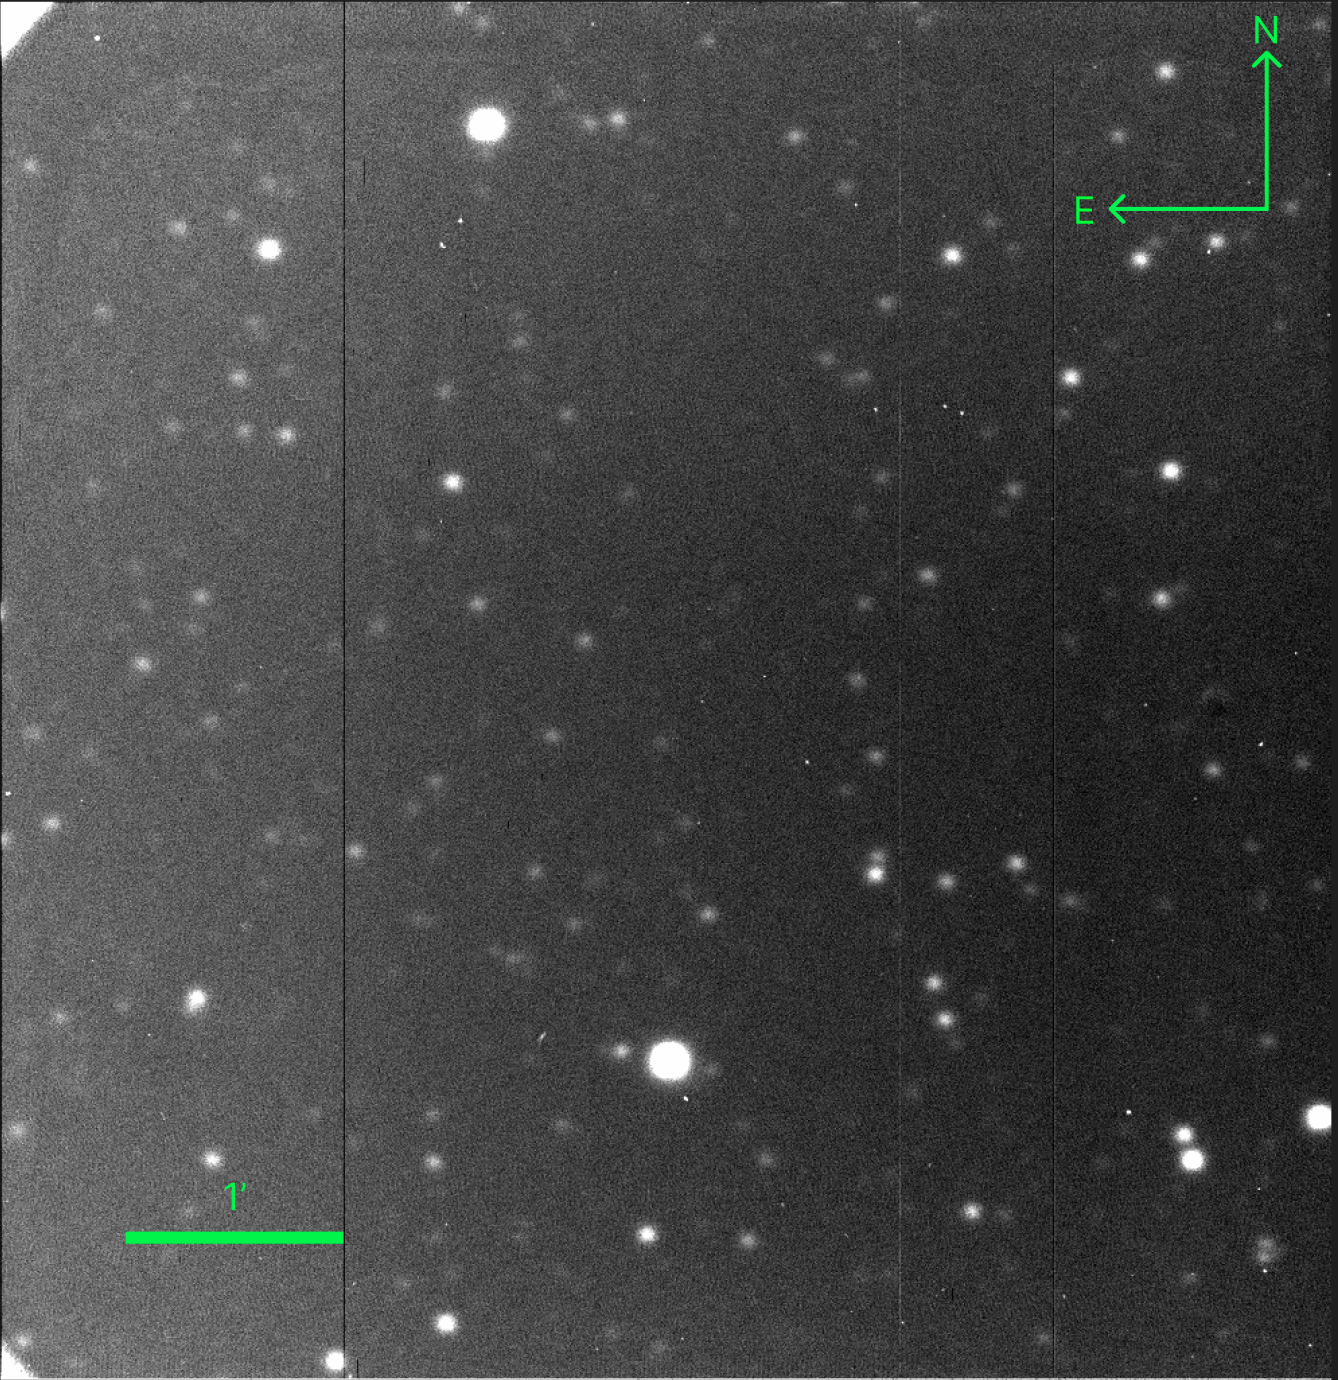
\includegraphics[width=\textwidth]{landB_scale.png}
            \caption[Landolt B]%
            {{\small Landolt B}}    
            \label{fig:landB}
        \end{subfigure}
        \hfill
        \begin{subfigure}[b]{0.475\textwidth}  
            \centering 
            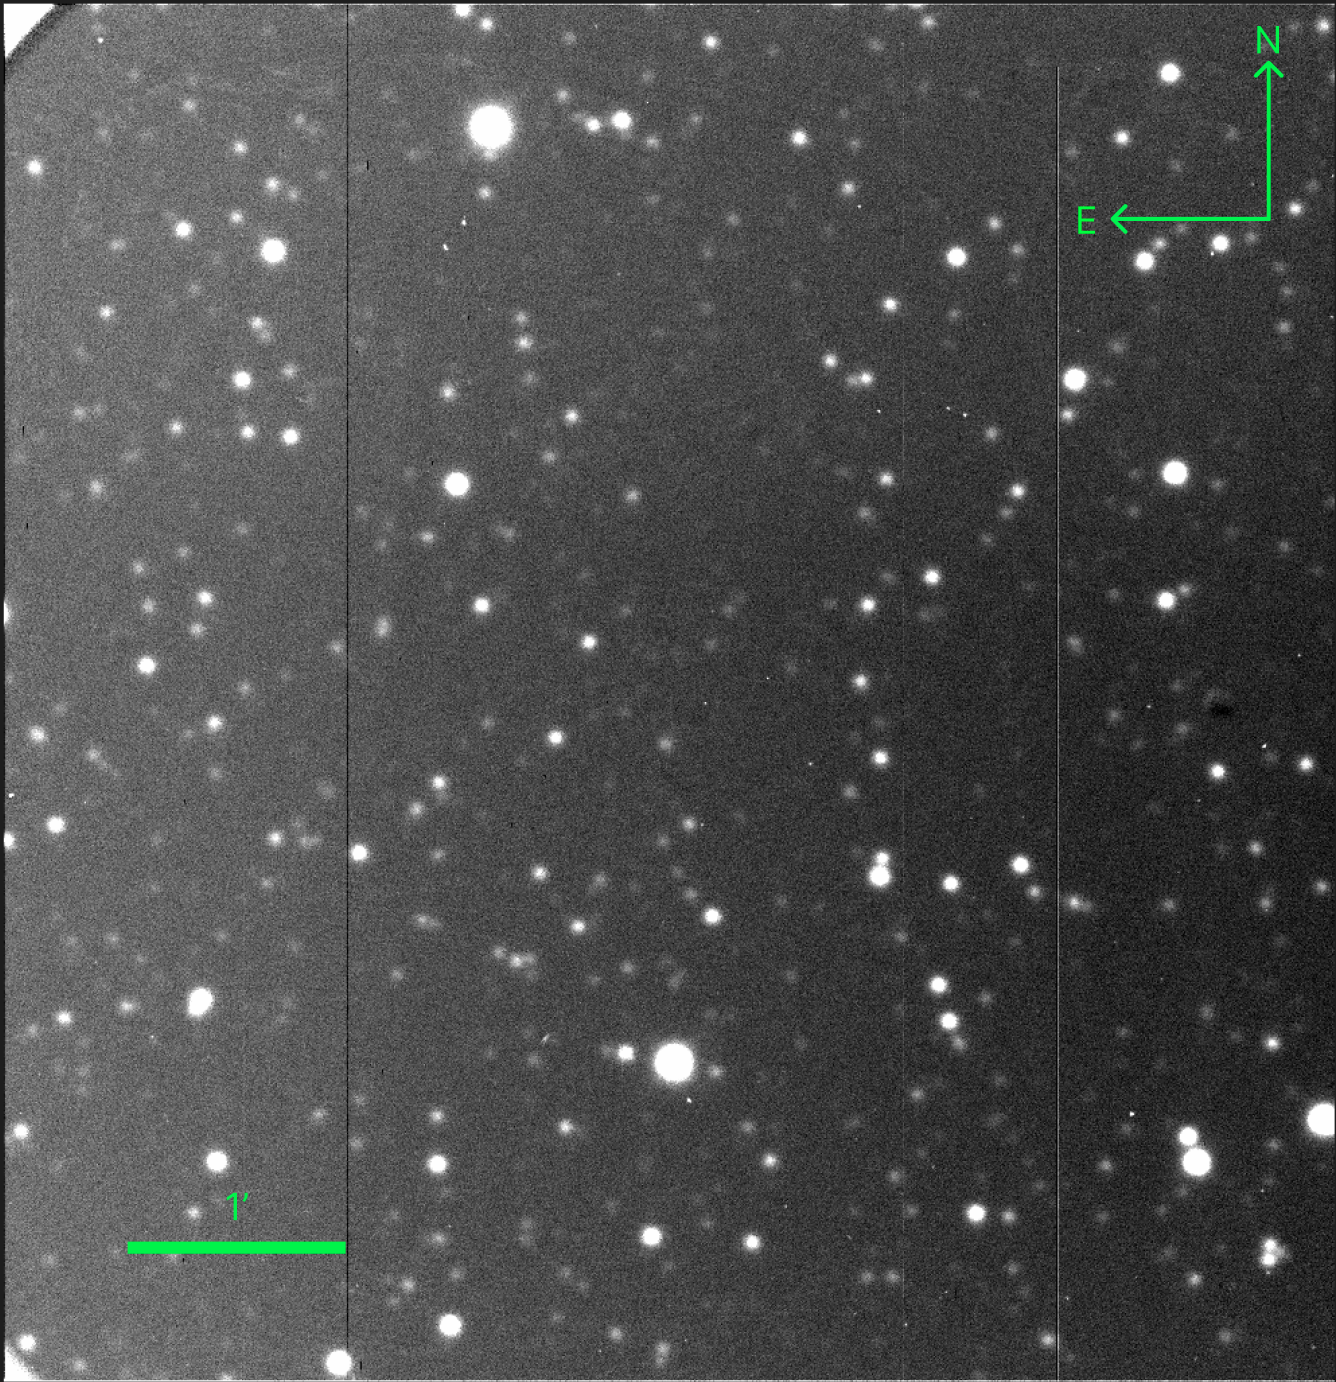
\includegraphics[width=\textwidth]{landV_scale.png}
            \caption[]%
            {{\small Landolt V}}    
            \label{fig:landV}
        \end{subfigure}
        \vskip\baselineskip
        \begin{subfigure}[b]{0.475\textwidth}   
            \centering 
            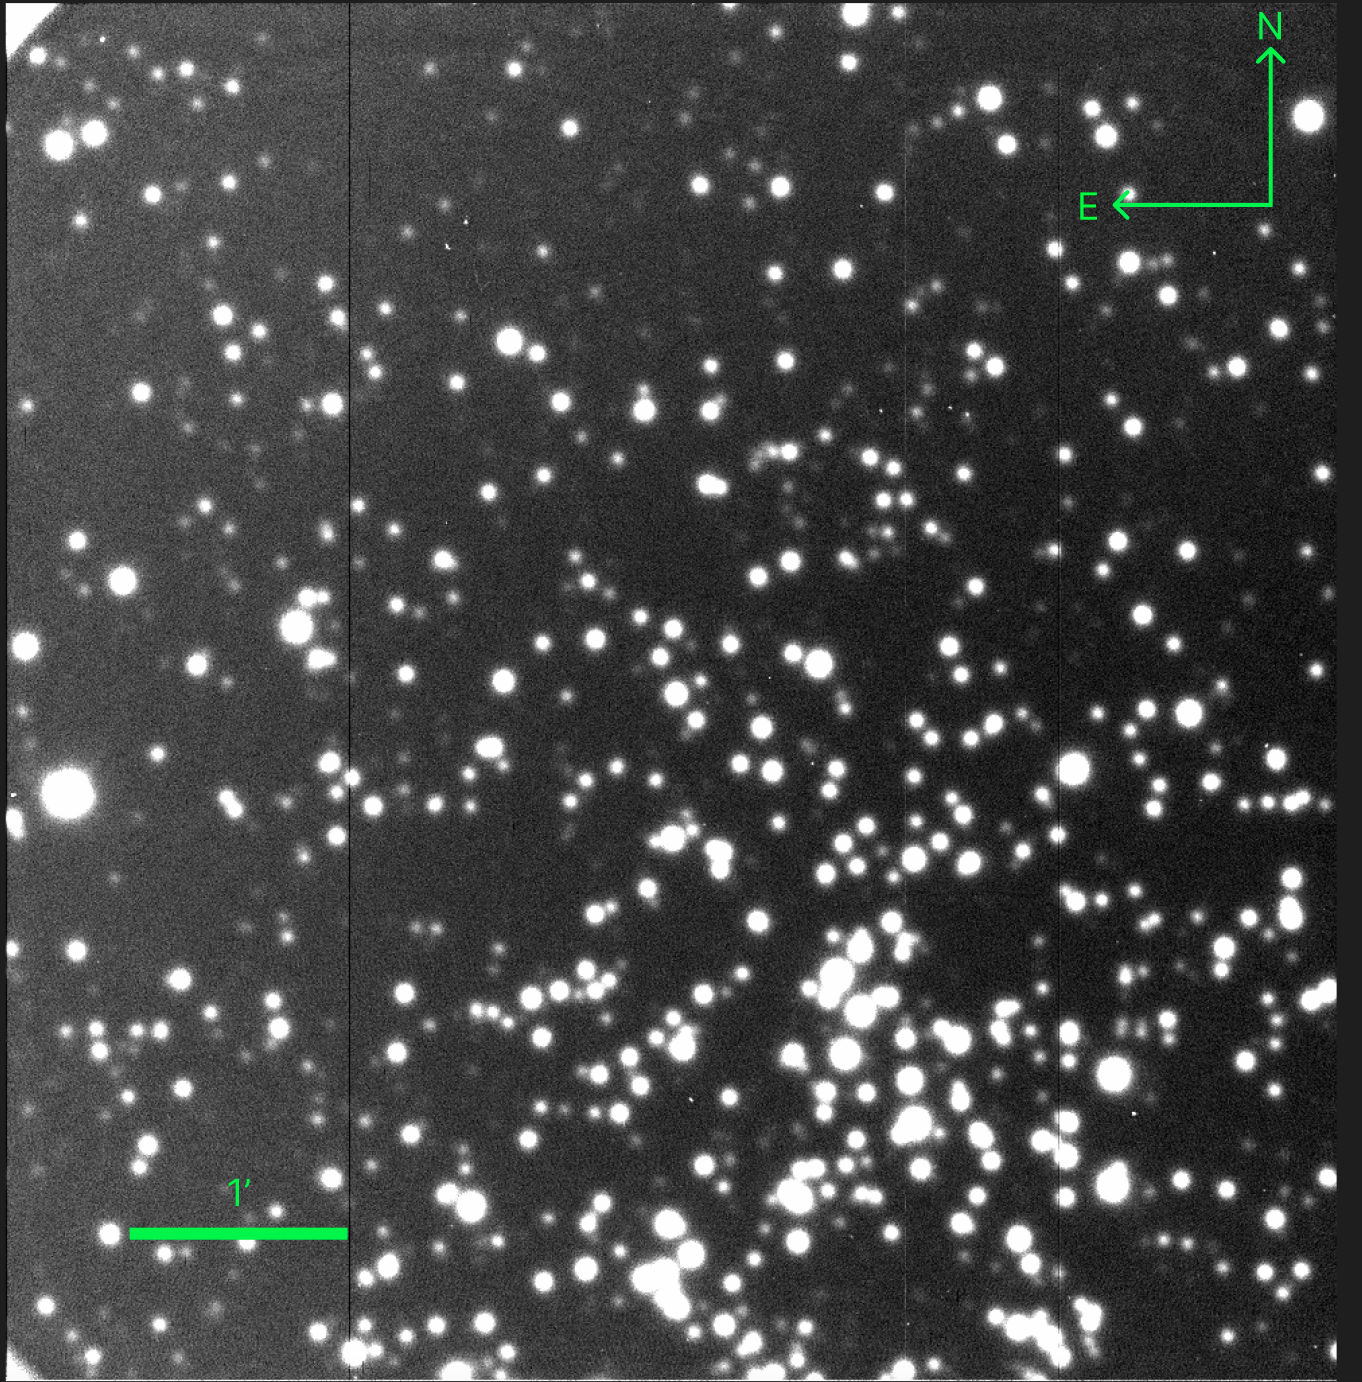
\includegraphics[width=\textwidth]{ngcB_scale.png}
            \caption[]%
            {{\small NGC B}}    
            \label{fig:ngcB}
        \end{subfigure}
        \hfill
        \begin{subfigure}[b]{0.475\textwidth}   
            \centering 
            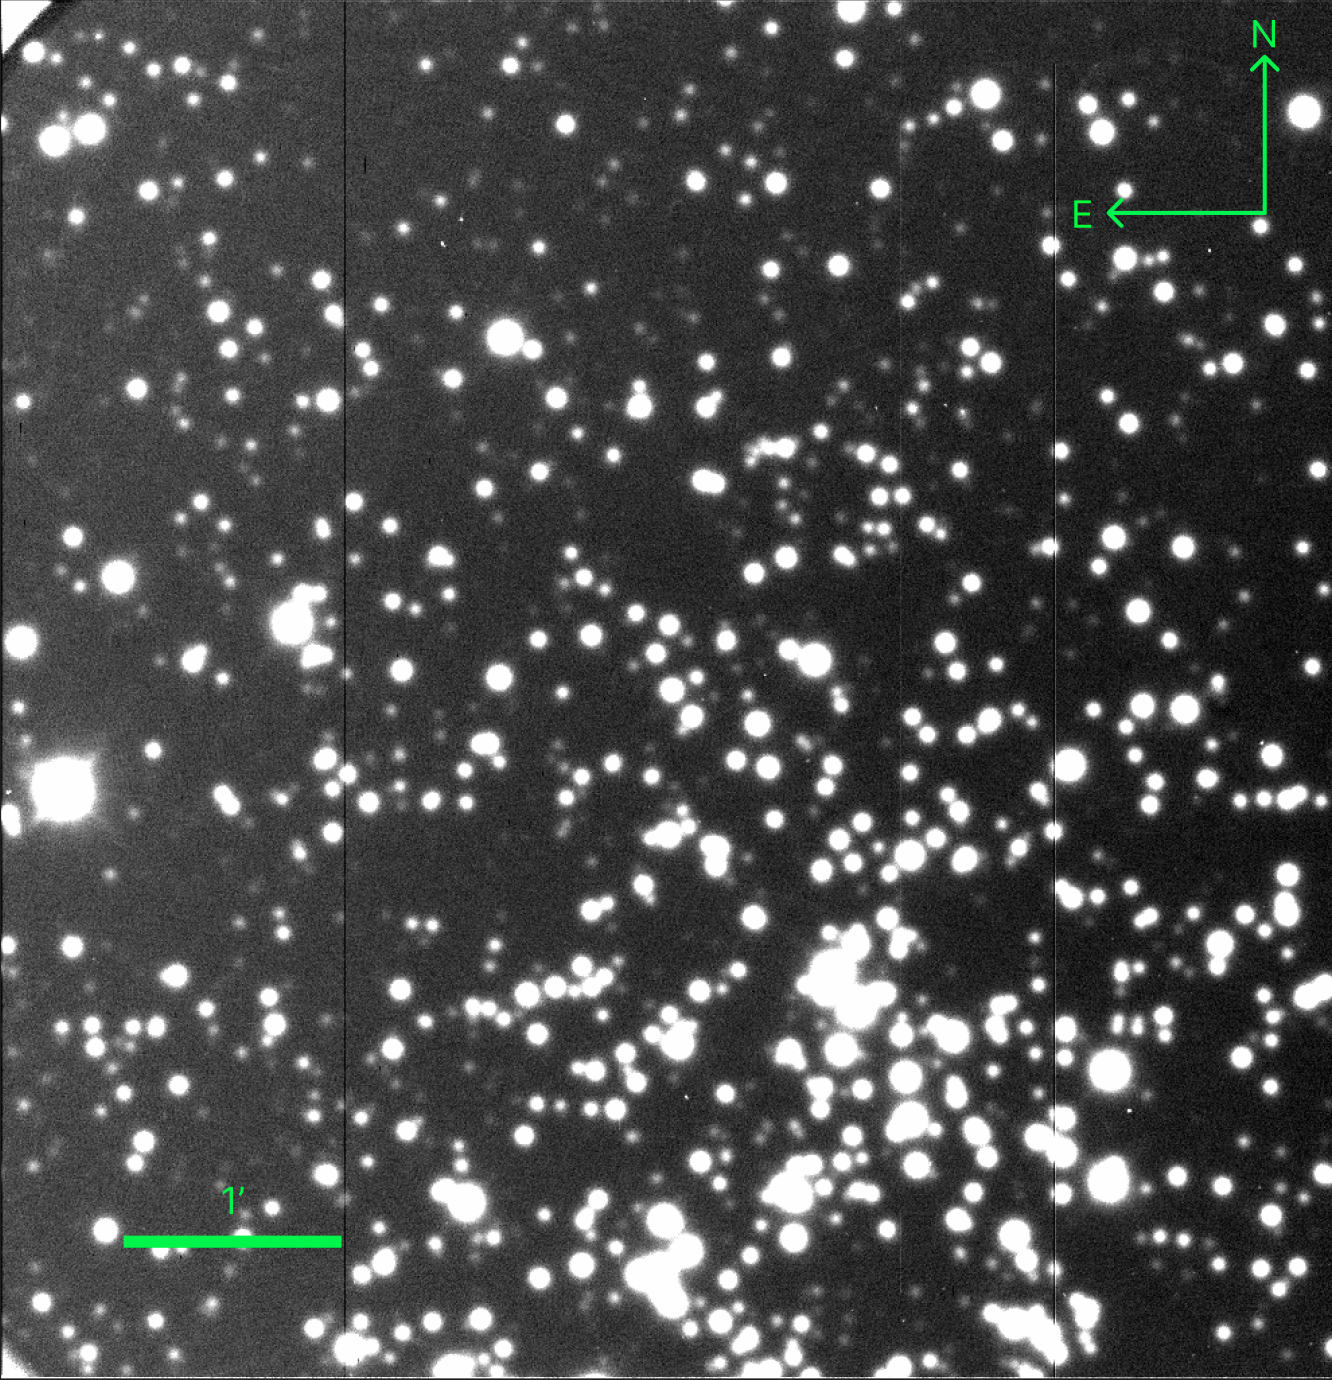
\includegraphics[width=\textwidth]{ngcV_scale.png}
            \caption[]%
            {{\small NGC V}}    
            \label{fig:ngcV}
        \end{subfigure}
        \caption[ The four reduced science images ]
        {\small Reduced science images} 
        \label{fig:sci}
    \end{figure*}

    We carried out aperture photometry using the \textit{photutils} Python package. We found star positions in both fields with only the B filter images using the \textit{DAOStarFinder().find\_stars} routine, with a threshold number of counts of 100 and a full-width at half-maximum of 3.26 px (derived from the estimated seeing of 1.2 arcsec converted to pixels). After background subtraction using \textit{photutils.MedianBackground}, aperture photometry was carried out using a circular aperture with a radius of 7 arcsec, to match the Landolt photometry.

    Using the counts per second $F_{L,i}/t_{int}$ (where $t_{int} = 60$) and the magnitudes $M_i$ of the Landolt star in both filters, we computed zero points:

    \begin{align}
        ZP_i = 2.5 \log_{10} \frac{F_{L_i}}{t_{int}} + M_i,
    \end{align}

    where $i = B, V$ to represent both filters. Using this, we divided the sums over each aperture by $t_{int}=60$ to get the counts per second, and computed the magnitude of each star in $B$ and $V$ using the zero-point:

    \begin{align}
        M_i = -2.5 \log_{10} \frac{F_{L_i}}{t_{int}} + ZP_i.
    \end{align}

    \section{Results}

    We computed zero-points of $ZP_B = 22.535, ZP_V = 22.740$. Using this, we computed magnitudes in $B$ and $V$ for each of the 146 identified targets and and plotted them in a color-magnitude diagram, shown in Figure~\ref{fig:hr}, with $V$ plotted against $B - V$. For clarity, we removed a single outlier at $(B - V = -3.55, V = 21.99)$.

    \begin{figure}
        \centering
        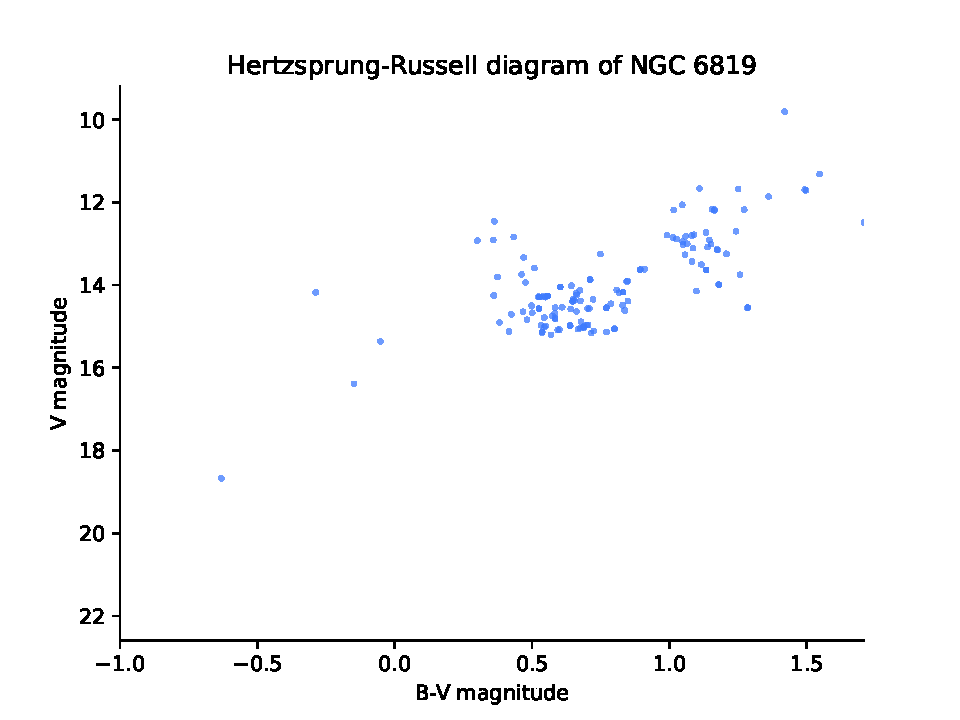
\includegraphics[width=0.8\textwidth]{hr_diagram.pdf}
        \caption{Hertzsprung-Russell diagram}
        \label{fig:hr}
    \end{figure}

    The figure shows a trend resembling a main sequence but not precisely the expected trend. This is likely due to different seeing than the 1.2 arcseconds assumed, which would result in a larger full-width at half-maximum and different sets of identified targets from photometry.

    We overplotted the Padova Stellar Evolution Isochrones, as computed by the CMD 3.6 stellar isochrone web interface\footnote{\href{http://stev.oapd.inaf.it/cgi-bin/cmd}{http://stev.oapd.inaf.it/cgi-bin/cmd}}, on the H-R diagram. The result is shown in Figure~\ref{fig:isochrones}. This indicates that the stars making up the cluster are between 100 Myr and 500 Myr old.

    \begin{figure}
        \centering
        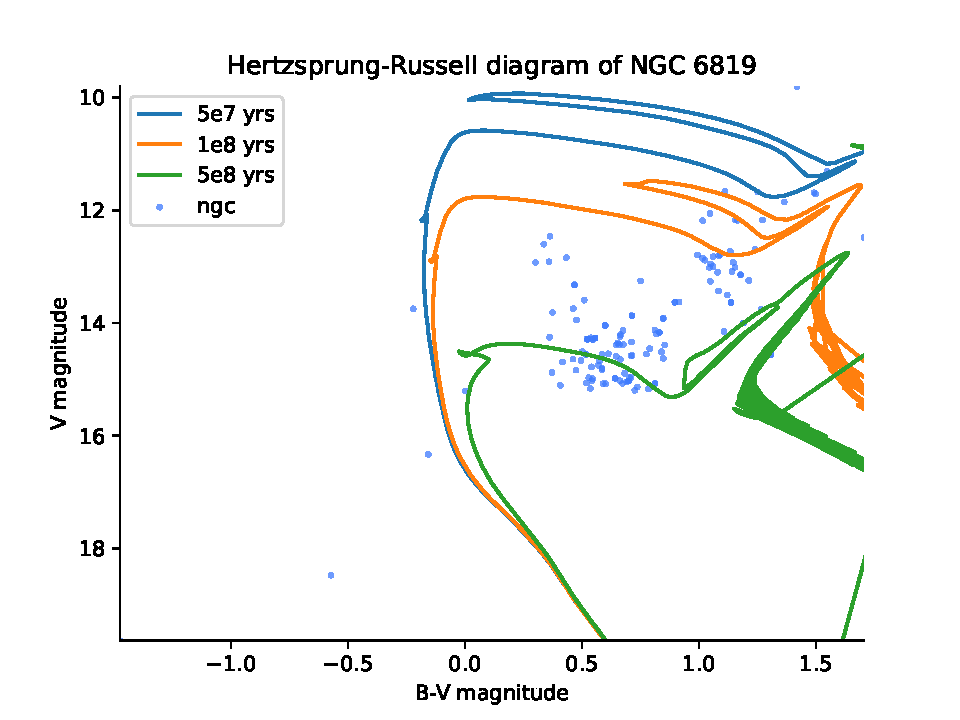
\includegraphics[width=0.8\textwidth]{isochrones.pdf}
        \caption{Hertzsprung-Russell diagram with isochrones overplotted}
        \label{fig:isochrones}
    \end{figure}

    The accepted age of NGC 6819 is $2.5 \pm 0.5$ Gyr, which implies the estimate here is off by an order of magnitude. This is likely due to the aforementioned issue with seeing, or due to insufficiently fine adjustment of the zero point of the isochrones.


\end{document}